\chapter{Interacciones con el blanco}

Esta clase tiene como objetivo familiarizarse con la interpretación visual de imágenes SAR. Para ello se estudiaran las interacciones de los distintos blancos para las bandas X, C y L.

\section{Interpretación visual}

En las microondas se suele hablar de tres grupos de interacciones: doble rebote, en volumen y especular, las cuales dependerán del blanco y la banda del satélite (Figura \ref{fig:interacciones}).

\begin{figure}[h!]
    \centering
    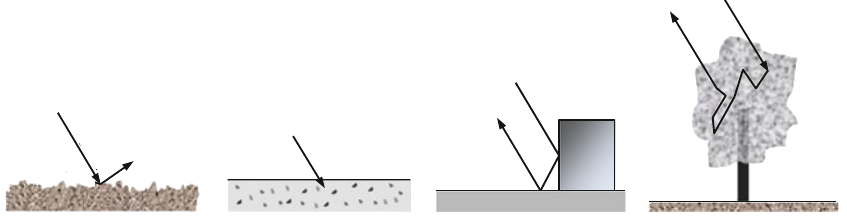
\includegraphics[width=0.5\textwidth]{fig:interacciones.png}
    \caption{Interacciónes con distintos blancos: -a- superficial, -b- subsuperficial, -c- doble rebote y -d- en volumen.}
    \label{fig:interacciones}
\end{figure}

\subsection{Banda-X}

Las imágenes adquiridas en \emph{Banda X} son las que tienen menor longitud de onda, por lo tanto tiene menos penetración en la vegetación y mayor backscatter en suelos sin cobertura (Figura \ref{fig:interacciones}).


Abra la imagen \directory{CSKS3\_GEC\_B\_S2\_03\_HH\_RD\_SF\_20141221211655\_20141221211703.h5} de la carpeta \directory{material/raster\_data>COSMO}. Despliege la banda \path{Sigma_HH_db}.

Utilice la imagen óptica para identificar:

\begin{enumerate}
    \item La pista de aterrizaje.
    \item Zonas urbanas.
    \item Zonas con vegetación.
    \item El agua que está en el lago.
    \item El agua del canal.
\end{enumerate}
Luego especifique en que colores los observa en la imágen SAR.
\begin{que}
    ¿A qué interacciones corresponde cada uno de los blancos enunciados anteriormente?
\end{que}

\subsection{Banda C}

Las imágenes adquiridas en \emph{Banda C} tienen longitudes de onda intermedias, entonces tendrán menos reflectancia en los suelos sin cobertura, dando información sobre el scattering en volumnes (Figura \ref{fig:interacciones}).

Abra la imagen \path{SENTINEL} de la carpeta \directory{material/raster\_data/SENTINEL1}. Despliege la banda \path{Sigma_HH_db}.

Utilice la imagen óptica para identificar:

\begin{enumerate}
    \item La pista de aterrizaje.
    \item Zonas urbanas.
    \item Zonas con vegetación.
    \item El agua que está en el lago.
    \item El agua del canal.
\end{enumerate}
Luego especifique en que colores los observa en la imágen SAR.
\end{enumerate}

\begin{que}
    ¿A qué interacciones corresponde cada uno de los blancos enunciados anteriormente?
\end{que}

\subsection{Banda L}

Las imágenes adquiridas en \emph{Banda L} son las que poseen mayor longitud de onda. En general, mantendrá interacciones especulares con los suelos sin cobertura, pudiendo penetrar en funcion del grado de humedad. Además, permitirá identificar propiedades de las coberturas vegetadas por debajo del canopeo (Figura \ref{fig:interacciones}).

Abra la imagen \path{ALOS} de la carpeta \directory{material/raster\_data/ALOS}. Despliege la banda \path{Sigma_HH_db}.


Utilice la imagen óptica para identificar:

\begin{enumerate}
    \item La pista de aterrizaje.
    \item Zonas urbanas.
    \item Zonas con vegetación.
    \item El agua que está en el lago.
    \item El agua del canal.
\end{enumerate}

\begin{que}
    ¿A qué interacciones corresponde cada uno de los blancos enunciados anteriormente?
\end{que}

\section{Valores de $dB$}

<<<<<<< HEAD
Es habitual expresar el valor del coeficiente de backscatter en dB para las imágenes SAR. Para calcularlo en distintos sectores de la imagen, puede posicionarse sobre un píxel y observar en \emph{Pixel info} el valor de \path{Sigma0_HH_db} en dB.

=======
Es habitual expresar el valor del coeficiente de backscatter en dB para las imágenes SAR. Para calcularlo en distintos sectores de la imagen puede posicionarse sobre un píxel y observar en \menu{Pixel info} el valor de \path{Sigma_HH_db} en dB.

Observe guiandose con la imagen óptica para la imagen \emph{COSMO}:
>>>>>>> 9cad12d80de0edb141987ff58af94e4c618cbd9f

Utilice la imagen óptica para identificar en la imagen \path{COSMO}:

 \begin{enumerate}
     \item El valor de dB de la pista de aterrizaje.
     \item El valor de dB de las zonas urbanas.
     \item El valor de dB de las zonas con vegetación.
     \item El valor de dB para el agua del lago.
     \item El valor de dB para el agua del canal.
 \end{enumerate}

<<<<<<< HEAD
Se puede calcular el valor promedio de dB seleccionando una región especifica en la imagen. En primer lugar, debe crear el contenedor del vector haciendo click en \emph{Vector, New Vector Data Container}. Nombrelo \emph{Urbano} (Figura \ref{fig:vector-cont}). Seleccione luego  \emph{Rectangle drawing tool} de la barra de herramienta y digitalice un rectángulo sobre la zona urbana. Para confirmar la geometría haga click fuera de ella.
=======
Otra forma de obtener estos valores es calculando el promedio sobre una región. Para esto haga click en \menu{Vector>New Vector Data Container} y ponga el nombre \emph{Úrbano} (Figura \ref{fig:vector-cont}). Seleccione luego la herramienta \menu{Rectangle drawing tool} de la barra de herramienta y digitalice un rectangulo sobre la zona úrbana. Para confirmar la geometría haga click fuera de ella luego de crearla
>>>>>>> 9cad12d80de0edb141987ff58af94e4c618cbd9f

\begin{figure}[h!]
    \centering
    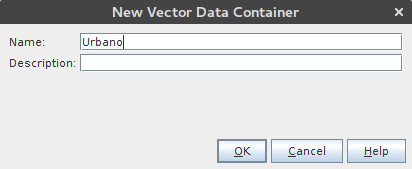
\includegraphics[scale=0.4]{fig:vector-cont.png}
    \caption{}
    \label{fig:vector-cont}
\end{figure}

Repita el proceso y cree contenedores de vectores para zonas de vegetación, agua con alto y bajo brillo y la pista de aterrizaje.

<<<<<<< HEAD
En el menú \emph{Analysis, Statistics} y tilde la opción \emph{Use ROI maks(s)} (Figura \ref{fig:estadistica}). Seleccione la región Urbano, haga click en el botón \emph{Refresh view} y el SNAP calculará la estadística. Puede hacerlo para varias regiones en simultaneo.
=======
Dirijase luego al menú \menu{Analysis>Statistics} y en la ventana que aparece tilde la opción \emph{Use ROI maks(s)} (Figura \ref{fig:estadistica}). Seleccione la región Urbano y haga click en el botón \emph{Refresh view}. El SNAP calculará la estadística para la zona y devolverá la estadística para la región seleccionada. Puede seleccionar varias regiones en simultaneo para calcular la estadística en cada una.
>>>>>>> 9cad12d80de0edb141987ff58af94e4c618cbd9f

\begin{figure}[h!]
    \centering
    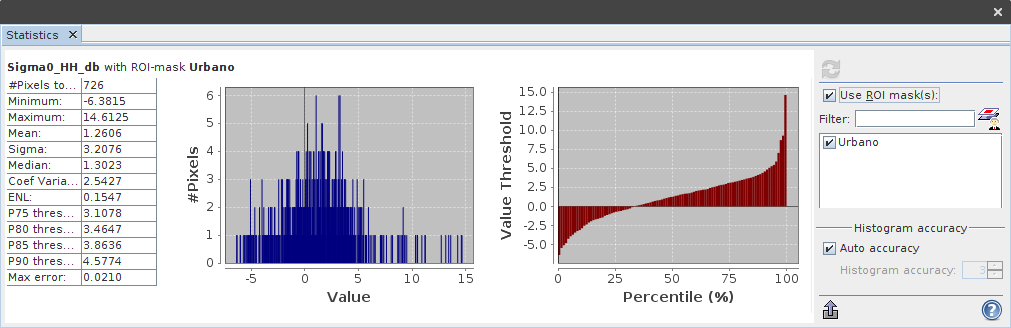
\includegraphics[scale=0.4]{fig:estadistica.png}
    \caption{}
    \label{fig:estadistica}
\end{figure}

Repita este análisis para las imágenes en banda L y C.

\section{Actividad}

Comparando las tres imágenes SAR utilizadas responda:

\begin{que}
    ¿Qué coberturas tienen siempre valores altos de brillo? ¿Cómo se puede interpretar la interacción?
\end{que}

\begin{que}
    ¿Qué coberturas tienen siempre valores bajos de brillo? ¿Como se puede interpretar la interacción?
\end{que}

\begin{que}
    ¿Cuál es la cobertura que más varía al cambiar de banda?
\end{que}

\begin{que}
    ¿Cuáles son las coberturas con más ruido dentro de las imágenes?
\end{que}

\begin{que}
    Observe las imágenes que no se encuentran en dB. ¿Qué diferencia encuentra en la distribución de valores de brillo?
\end{que}
